\chapter{Introduction}

The purpose of this chapter is to transform a scientifically literate reader who may be vaguely familiar with the idea of a ``quark'' into one who can understand the motivation and techniques behind the analysis presented in the rest of this thesis. 
If you are an extremely educated physicist who regularly performs lattice quantum chromodynamics calculations in their head, I would also encourage you to read this chapter it its entirety as it may contain egregious errors that need to be corrected. 

\section{What is fundamental?}
The answer to the question ``What are the fundamental building blocks of our universe?'' has changed drastically over the course of human history.
The idea that all matter is composed of smaller, uncuttable pieces has been around since 5th century BCE when Greek philosophers Democritus and Leucippus first introduced the concept of an atom\cite{}. 
While this idea was initially ignored in favor of more theological descriptions of our universe, over the span of a millennium or two the atom became the de facto indivisible building block of nature. 
However, everything changed around the turn of the 20th century when scientists like Rutherford and Chadwick determined that the supposedly indivisible atom was composed of even smaller particles, eventually named protons and neutrons. 
The notion that protons and neutrons were unbreakable was relatively short lived, as not even half a century later the deep inelastic scattering experiments performed by Kendall, Friedman and Taylor revealed that protons (and subsequently neutrons) were actually composed of even smaller particles, dubbed ``partons''. \cite{}
This discovery was one of the largest contributing factors to the creation of the so-called Standard Model of particle physics, a theory which describes all of the fundamental particles and the way in which they interact with each other. A diagram of those fundamental particles can be seen in Figure 1.1.
\begin{figure}
    \centering
    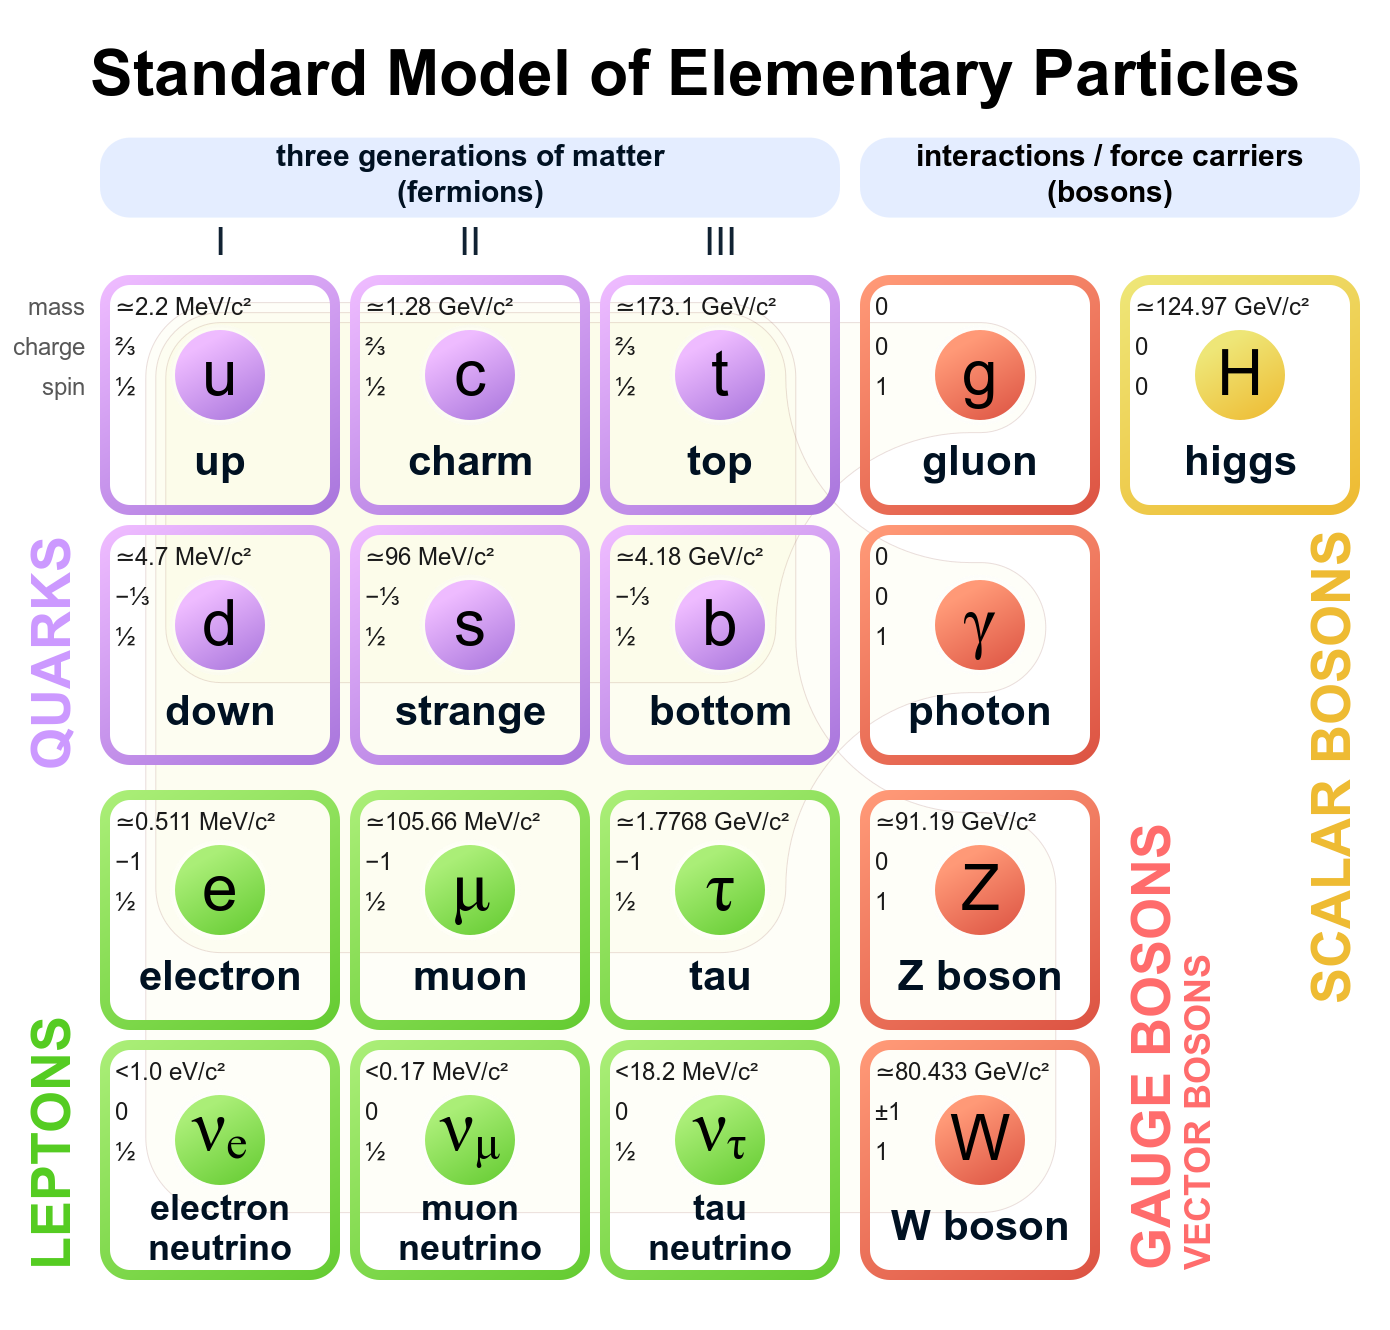
\includegraphics[scale=0.2]{figures/StandardModel.png}
    \caption{A diagram depicting the particles we currently believe are fundamental within the so-called ``Standard Model'' of particle physics.}
    \label{fig:my_label}
\end{figure}
 It should be noted that all of the particles labeled as quarks and leptons -- collectively as ``fermions'' -- have corresponding anti-particles with opposite electric charge.
The equation that describes all of these particles and their interactions, often incorrectly\footnote[1]{It is ``incorrect'' because this is technically a Lagrangian density (i.e. Lagrangian per unit volume), but as it is usually integrated over all space the distinction is mostly irrelevant.} referred to as the ``Standard Model Lagrangian'', can be compactified into a relatively palatable form that can easily fit on a coffee cup like the one shown in Figure 1.2.
\begin{figure}
    \centering
    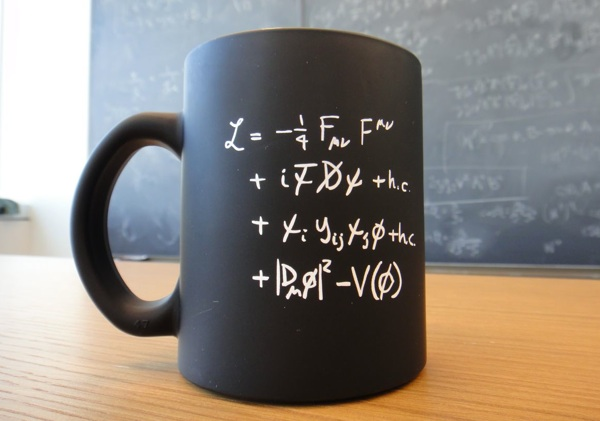
\includegraphics[scale=0.5]{figures/StandardModelCup.jpg}
    \caption{A coffee cup with the Standard Model Lagrangian density printed on its side. Please ignore the ``+ h.c.'' term following the $i\Bar{\psi}\slashed{D}\psi$, it is the result of a small lapse in judgement from the mug makers.}
    \label{fig:my_label}
\end{figure}

While this equation may appear brief\footnote{Here ``brief'' is in the eye of the beholder, but certainly its brevity is misleading as even in the first line the $F_{\mu\nu}$ refers to three completely different gauge field tensors...}, it can be used to completely describe three of the four fundamental forces of nature: 
\begin{enumerate}
    \item The Electromagnetic Force, which is responsible for the electrons pushing against each other to keep you from falling through your chair,
    \item The Weak Nuclear Force,  which is responsible for the initiating the nuclear fusion reactions that fuel our sun, and 
    \item The Strong Nuclear Force,  which is responsible for holding quarks and gluons together in bound stands known as hadrons, like the protons and neutrons that make up everyday matter.
\end{enumerate}
The only fundamental force missing from this list is the Gravitational Force, which is described by a completely separate set of equations\footnote{Specifically, the Einstein Field Equations, $G_{\mu\nu} + \Lambda g_{\mu\nu} = \kappa T_{\mu\nu}$, but this is the thesis of a particle physicist so gravity is taboo.}

Each of the three forces that are described within the Standard Model are mediated by different gauge bosons. For example, the electromagnetic force is mediated by the boson known as the photon, the weak nuclear force is mediated by the W and Z bosons, and the strong nuclear force is mediated by bosons known as gluons. 
In this thesis we will be primarily focusing on the Strong Nuclear Force, which acts solely on particles with color charge -- an intrinsic property of quarks and gluons. 
The ``color'' charges are red, green, and blue with antio


Even though each of the electromagnetic, weak and strong forces can be described using the Standard Model Lagrangian, the way in which they appear within the equation is not easy to determine.
For example, the electromagnetic force actually corresponds to line 1
